\chapter{Related Work}


boilerplate text, boilerplate text, boilerplate text, boilerplate text, boilerplate text, boilerplate text, boilerplate text, boilerplate text, boilerplate text, boilerplate text.


\section{Blockchain Basics}

The concept of a blockchain was introduced in the form of published hashes of data in newspaper format  \cite{whitakerArtBlockchainPrimer2019}

\subsection{Consensus Algorithms}

Proof-of-Work

Proof-of-Stake


\subsection{Oracles}



\subsection{Non-Fungible Tokens}

Created by crypto-kitties in 2018, specifically for art, but protocol can be used for other applications.



\section{Existing Repositories}

\subsection{Rhizome ArtBase}



\section{Crypto-Art}


Early bitcoin inscribed ASCII artworks.

McCoy early work on Namecoin (2014)

Early work by Rhea Myers, predates NFTs.

Rhea Myers "Token Equals Text" (2019)


Tezos as the art chain (mention participation in basel

\section{Digital Art Preservation}

\subsection{NDSA Levels of Digital Preservation}


\begin{table}[h!]
\centering
\captionsetup{type=table} % This makes the caption be treated as a table caption
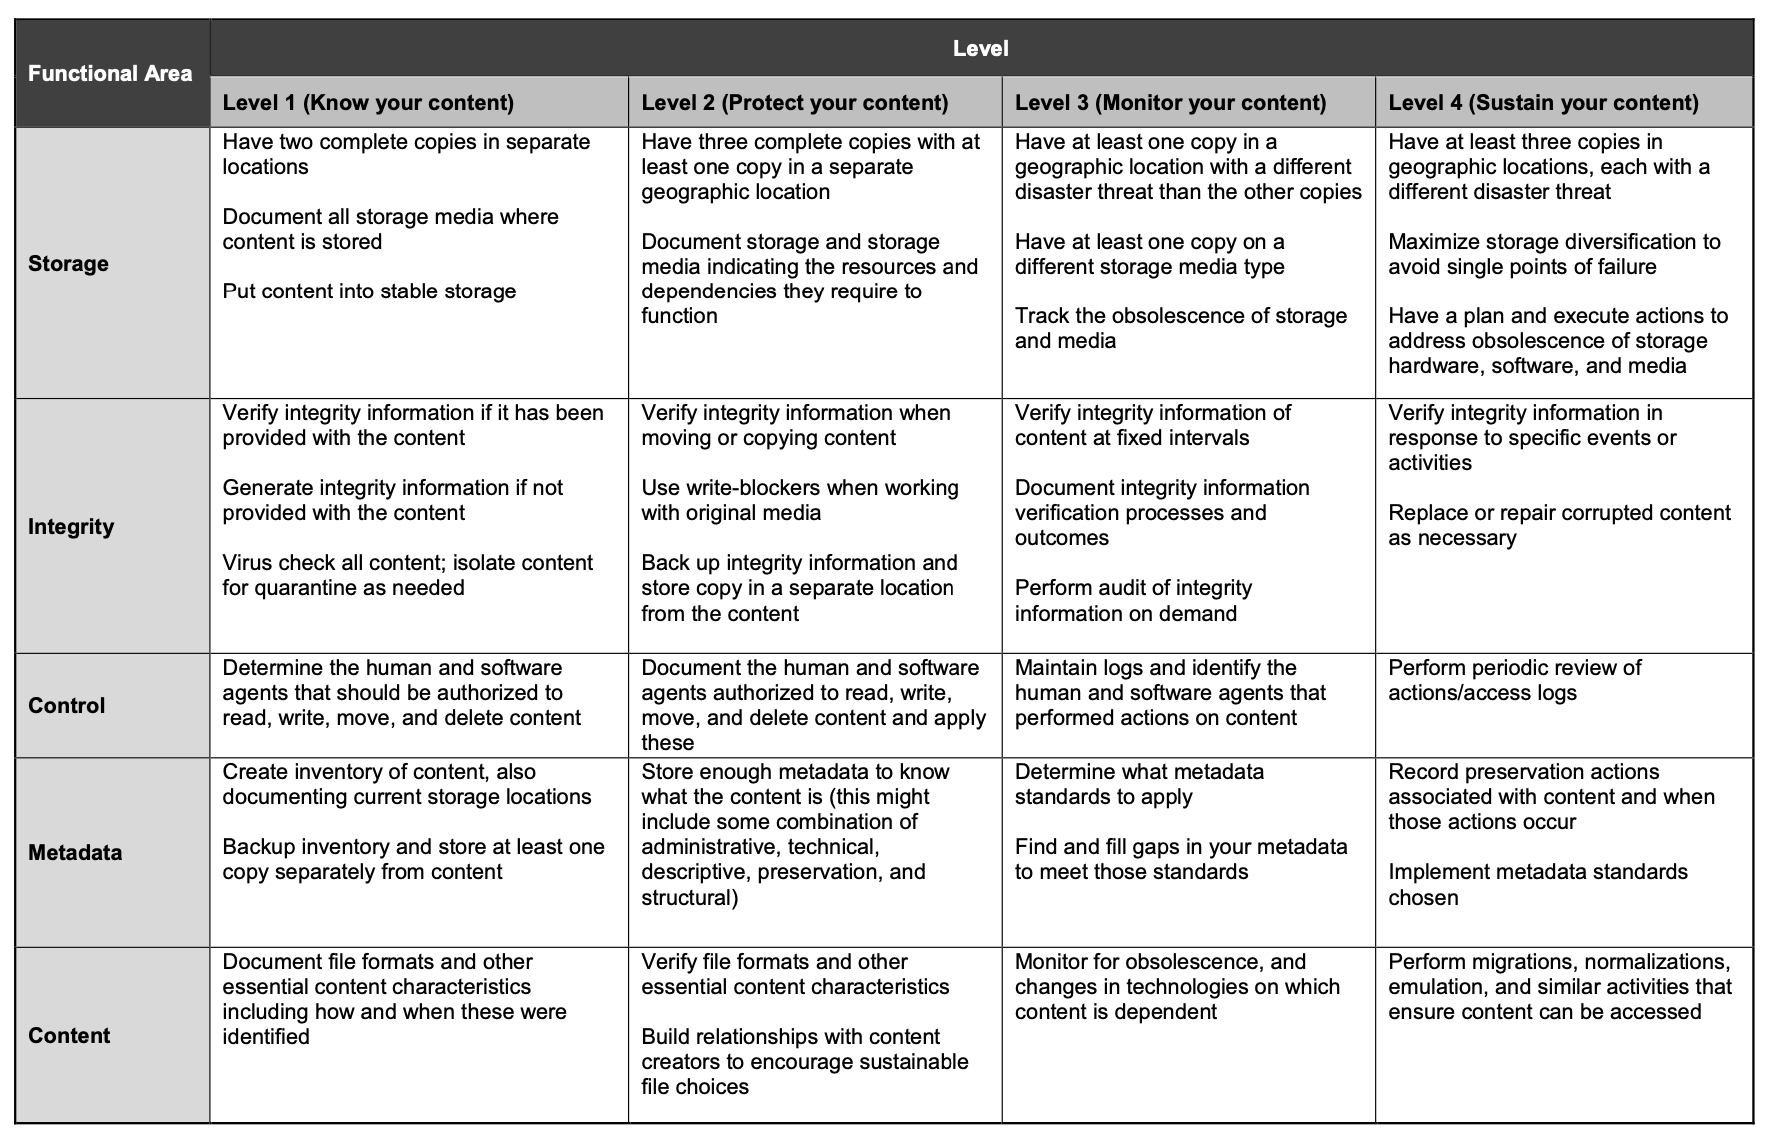
\includegraphics[width=\textwidth]{table-ndsa-matrix.png} % Adjust the width as needed
\caption[NDSA Levels of Digital Preservation Matrix V2.0]{NDSA Levels of Digital Preservation Matrix V2.0. Source: https://osf.io/qd54c}
\label{tab:ndsa-levels-of-digital-preservation}
\end{table}


\section{Web Archiving: State of the Art}

webrecorder
\subsection{Web Archiving Standards}

WARC


\section{Data Storage}

\subsection{On-Chain Storage}


mention fxhash articles (https://docs.fxhash.xyz/articles) and their tezos pointer scheme (https://github.com/fxhash/specifications/blob/main/general/tezos-storage-pointers.md) which may be useful for the idea of cross contract references, which is my plan for documentation (each person, one contract, cross-referecning OBJKTs)

\subsection{Interplanetary File System (IPFS)}

\subsection{Arweave}




\section{Provenance}

\subsection{Atomic Form}

Atomic Form combines the best of IPFS and Arweave into a single solution \cite{maneliusExtendingNFTMetadata2024}




\section{Interactivity}

\subsection{Self-Awareness}

\begin{figure}[h]
    \centering
    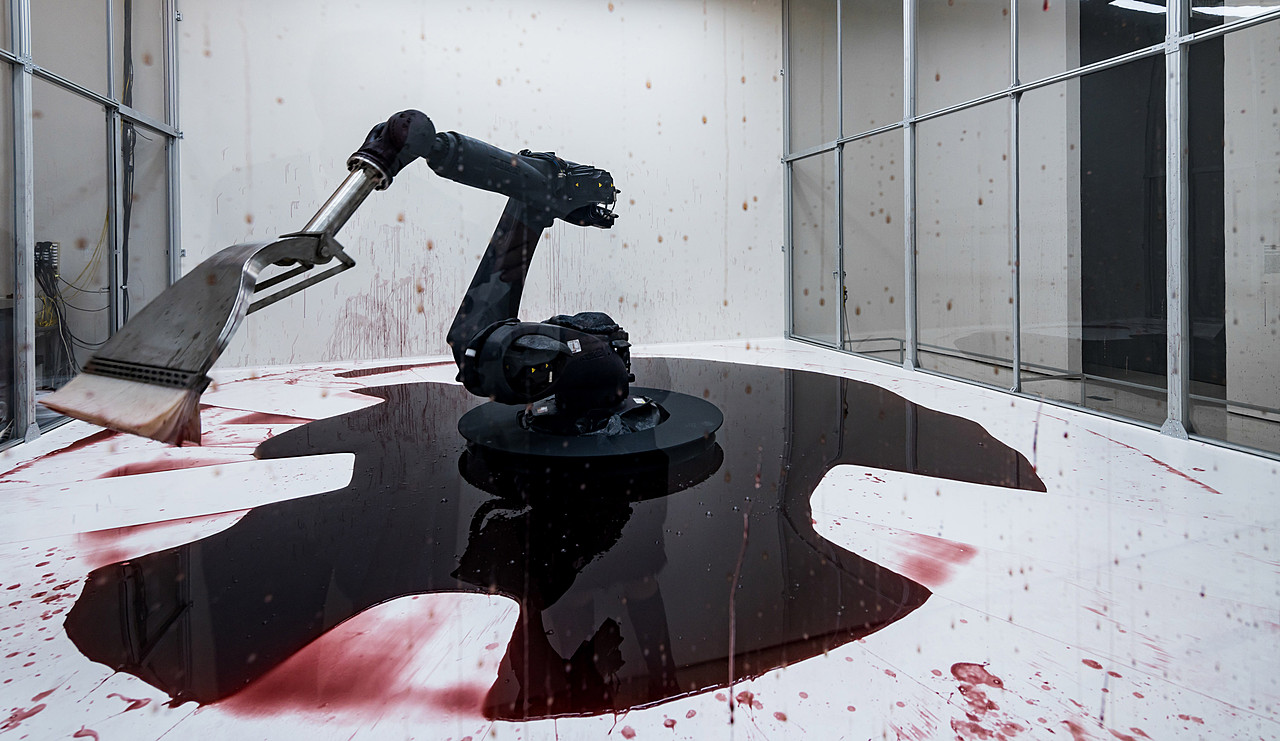
\includegraphics[width=\linewidth]{artwork-robot-cant-help.jpg}
    \caption[Can’t Help Myself by Sun Yuan \& Peng Yu]{Can’t Help Myself by Sun Yuan \& Peng Yu, 2016. Source: https://www.guggenheim.org/artwork/34812}
    \label{fig:robot-canthelp}
\end{figure}


This is a test reference to the work \cref{fig:robot-canthelp}

\subsection{Viewer Interactivity}

\subsection{Network Interactivity}

\subsection{Time Interactivity}


\subsection{LocalStorage Interactivity}

Entanglement by Bjork (have permission for screenshots)

\section{Determinism}

This section deals with whether artworks are deterministic in the way they are rendered or whether there is an element of randomness that even given all the same starting conditions, the artwork will look very different each time. This categorisation is important for conservation because a nondeterministic artwork will be dificult to monitor from a browser obsolescence point of view, especially when using image difference between consecutive snapshots of the artwork. In the case of a non-deterministic artwork, the snapshots will be so different that they become ineffective in detecting changes due to browser version upgrades or other changes in web specifications overtime. In this context, the challenge is to differentiate between a deterministic animated artwork, and a nondeterministic artwork. This challenge exists, because even if an artwork is deterministic, unless there is a way to snapshot the exact same frame across all the snapshots then any image difference comparisons will result in exaggerated differences. In this case we may need to employ more advanced animation frame comparison algorithms, such that the sequence of the animation can be compared across snapshots, and these may involve the recording of the animation, rather than just taking a single snapshot in time. Of course, such a strategy has trade-offs, and in this particular case the trade-off would be a much larger snapshot file size, which will then impact on the overall economic sustainability of the archive.


\section{Code Security}

In this section I review methods of detecting potential malicious code

Strategies can involve code similarity checks \cite{ragkhitwetsagulComparisonCodeSimilarity2018} and particularly in JavaScript \cite{alfagehCloneDetectionTechniques2020} where an artwork's code can be compared against well known wallet code.

This can also aid in identifying potential outdated libraries which could contain vulnerabilities or even current libraries which were attacked by hackers, looking to add backdoors or other crypto exploiting code.



\section{Blockchain as the Medium}

Mad Dog Jones Replicator (2021) - uses an off-chain server (under control of the artist) as an oracle which sends "paper-jam" events to the artwork's smart contract.

\section{Decentralisation}
\label{sec:lit_review:decentralisation}

\section{Main Issues}

\subsection{Scalability}

One key aspect to remember is that adding more nodes to a network does not improve network scalability if each node must replicate the exact same computation as every other node, which is the case with most consensus and block validating nodes on a blockchain. Of course such wide replication of computation is still desired, for decentralisation purposes, as discussed in \ref{sec:lit_review:decentralisation}


\subsubsection{Moore's Law and Data Storage}

\section{Economic Sustainability}

mention VDP, its role in wg3.2 (beneficiaries), and how the idea spread to other marketplaces (https://docs.fxhash.xyz/pricing-and-supply)




\section{Stuff copied from prev chapter}





If art typically already follows, adapts to and reflects technological advances, the opposite cannot be said to happen. One goal of this project is to avoid approaching the issue of \emph{infrastructure} versus \emph{art} as separate things, but rather as a symbiotic relationship where the art and the infrastructure on which it relies complement and inform each other. This means a significant effort was made to study the evolution of digital art in general, with a special focus on netart. 

Prior to blockchain, the print medium was the most reliable way to archive and record one's work, and to build a reference-able portfolio. (Violet Bond in ``The Artist Toolbox'' feat @inWarhol and why being in print matters - https://twitter.com/i/spaces/1OwxWwAPnPkxQ?s=20 )

It is somewhat ironic, that hand prints and other rudimentary paintings on the walls of caves by our pre-historic ancestors are inherently more resilient to degradation than state-of-the-art digital art. We could argue that complexity is the enemy of conservation.


\section{Crypto Culture}


Crypto attempts to replace hierarchical systems of power, where rules are ultimately enforced by the use of violence, which a non-hierarchical system where ``good'' and ``bad'' behaviours are encouraged or discouraged via economic incentives and/or penalties.



\subsection{Social Contracts, Immutability and Hard Forks}


\todo : explain why I changed my stance on code is law.

This section will focus on one of crypto's core \emph{raisons d'être}, trustlessness.

The term trustlessness, does not mean untrustworthy. Rather it represent's an effort to make trust obsolete, replacing it with transparency and a-priory agreed social contracts. These social contracts, represented by code, both at the blockchain protocol level, as well as written into smart contracts, become immutable agreements, and self-executing rules of engagement. This concept is so deeply engrained into the crypto culture that any scenarios that rely on individual's trustworthiness are only considered when absolutely unavoidable.

Smart contracts play an important role in this concept, because once instantiated in a blockchain they become, by default, immutable. Participants that rely on the smart contract still need to verify that the code does what it is supposed to, and unintended and hard-to-find bugs are not only possible but unfortunately a common occurrence in this early stage of the smart contract industry. Even though these bugs can be exploited, leading to consequences which run counter to the intended social contract, the crypto community accepts this risk and tries to mitigate it with stricter contract development processes, and reviews and verifications. However, a smart contract which is purposefully designed to be mutable (a possibility under some circumstances) or which gives its creator or administrator powers that would require trust by the community on them, are naturally seen with suspicion and even counter to the accepted crypto culture values. In the early days of \indexglossary{ethereum} a name was given to this type of code-based social contract: rule of code.

An important feature of immutable social contracts is that they prevent, or at least minimise, the unilateral ``cheating'' by any participant in a transaction or a serie of transactions. In crypto, the act of cheating other participants is called a ``rug pull'', which means the symbolic act of ``pulling the rug out from under the feet of the victims'' leaving them off-balance and causing them to fall.

Immutability, however, does bring some inconveniences. Some times the immutable code fails to represent the expectation of the social contract, and this can happen for a number of reasons. For example, the code could have an unforeseen consequence due to a bug. Other times the needs of the community change with time and the social consensus evolves in ways which are incompatible with the original code. In some cases this evolution can even cause major fissures in the community, leading to a breakup in consensus, with major splits in the opinion of the best way forward. In these cases the immutable code is unable to adapt to a new reality, and the community has no option but to leave behind the original protocol, and jump to a new, modified protocol. We call this phenomenon a \emph{hard-fork}.

There were notable hard-forks in the history of crypto (mention BTC/BCH, ETH/ETC, etc)

Perhaps most importantly is that every participant in an activity is satisfied that their expectations are met by the system, and where opinions between them evolve and diverge, that the system provides a satisfactory and fair resolution to all stakeholders. 

\subsection{Why Decentralisation?}
(looking for a better heading. why do we need trustllessness, immutabilty, censorship resistence, etc)

Activism through digital art, see \cite[p.~212]{hopeDigitalArtsIntroduction2014} , benefits greatly from low barriers of entry, lack of gatekeepers, and censorship resistance (both as infra resilience, and social structures), but how can it be counter-balanced with curation of content, policing of copy mints or copyright infringement, removal of illegal material (i.e. child porn, etc).

Decentralisation as a way to remove single-points-of-failure, thus resilience to attack, was an intentional design decision of ARPANET, which led to the Internet we know today. \cite[p.10]{paulDigitalArt2015}



\section{A New Type of Art}

This thesis invites readers to look at networked art under a new light of sensorship-resistant long-lived preservation, powered by decentralised technologies. Rather than create its own visual aesthetic, this new kind of art may be characterised by a common set of processes and underlying architectures that afford it with the kind of long-lasting characteristic that is seldom attributed to digital medium art.
Another factor that distinguishes it from previous net art is the ability of art pieces to be ``aware'' of their own existence in the marketplace, allowing them to react to actions such as being put up for sale, being sold, the monetary amounts involved, who owns them, etc.
In theory, a piece of art could be created in such a way as to 'earn' a stipend from each sale, and through its own trading activity eventually earn enough as to be able to 'purchase' itself from its human owners, and gain some sort of freedom, or emancipation.
Futhermore, it attempts to blend the seemingly conflicting forces of preservation and evolution.

\subsection{Art as Revolution}

``If revolution can give art its soul, then art can give revolution its mouthpiece'' - Anatoly Lunacharsky

TODO: Refer to ``Art and Revolutio'' by Gerald Raunig (available in UMAC lib: NX 180 R45 Rau 2007)

Walter Benjamin hailed the liberatory and transformative effects of mechanical reproduction on art, suggesting that ``mechanical reproduction erodes the 'aura' of a work of art, which results from its unique existence in a time and place, which revolutionized the social function of art and allowed it to be used for politics rather than ritual''. (Benjamin, 2002: 103-6 - cited in \cite[p.3]{gereArtTimeTechnology2006}

\section{Contributions}

This thesis contributes to the body of knowledge in the following ways:

It proposes a new taxonomy for categorizing xxx which takes into account yyy, and zzz.

Using this new taxonomy an extensive review and categorization of xxx was undertaken and is available online at https://abc.xyz

It contributes to the field of digital art preservation by combining xxx with yyy in a novel way, and provides evidence of its efficacy in findings nnn.

It demonstrates de economic viability of running decentralised infrastructure by incentivising xxx via the use of zzz, as seen in chapter yyy.

In the field of information systems, it studies and reports on the application of xxx and yyy in the context of zzzz

In conducting the research, the efficacy of using methodology xxx was tested in the context of uuu, revealing limitations yyy and zzz.

Last but not least, it proposed a new paradigm for art creation based on xxx, and extensively tested its limitations. In doing so, it also raised important questions that should inform future research efforts. Namely, xxxx.

Digital assets like \gls{nonfungibletoken} are transforming the art world. An \indexacronym{nft} is a unique digital asset verified using blockchain technology.
This document discusses various examples (EX) of digital assets and their conservation techniques. This is the nature of the \gls{nonfungibletoken}.


\section{Conservation}

Mention how the Internet Archive, in cooperation with the MAME project, which started as an emulator for old arcade games, has now branched to include other kinds of vintage hardware, like consoles and even scientific calculators. \cite{scottjasonCalculatedMoveCalculators2023}

This is a quick mention of \gls{emulation} so that it appears on the glossary.


\subsection{Historical Consensus - Conservation of Bugs}

One interesting side-effect of maintain global consensus is that every full node must independently validate the whole chain, from it's genesis block until the latest block, which is commonly called the ``head'' of the blockchain. This means every full node, no matter how recently implemented, must be able to replicate every historical consensus rule, including any bugs in early node software, such that all historical block validation proceeds exactly as it did originally. Failure to replicate such bugs would potentially result in modern nodes considering historical blocks as invalid, hence refusing to follow the main historical chain and therefore forking the chain.


\section{Blockchain Interactivity}



\subsection{Burn it: NFTs as reedemable vouchers}

One of the most common interactions between collectors and projects is the act of collecting and burning tokens as a way to unlock other features in the project, access special drops, or others. Collectors have to weigh in the cost-opportunity of destroying a token in exchange for another which may, or may not, be more desirable for them, both from an economic and aesthetical point of view. Whilst creating an environment of engagement and gamification of the project, it can certainly be considered one of the most striking examples of commodification or art in the NFT world. The very act of permanently disposing of a piece of art in return for some kind of utility is arguably against the very ethos of ``art'' (that which has no utility).

The topic of utility has itself generated a fair amount of debate among the cryptoart enthusiasts. TODO: expand on this.

\subsection{Bootloader method}

A web3 approach is to load a lightweight bootloader OBJKT, which is able to contact the blockchain for the IPFS hash of the latest version of the artwork.

\begin{figure}[H]
  \centering
    \scalebox{1}
    {  \begin{sequencediagram}
    \newinst{browser}{\shortstack{User \\ Browser }}{}
    \newinst{marketUI}{\shortstack{Marketplace \\ UI }}{}
    \newinst{indexer}{\shortstack{Blockchain \\  Indexer }}{}    
    \newinst{ipfs}{\shortstack{IPFS \\  Gateway}}{} 
    \begin{call}{browser}{ }{marketUI}{1. page UI}
    \end{call}
    \begin{call}{browser}{ }{indexer}{2. OBJKT metadata}
    \end{call}
    \begin{call}{browser}{ }{ipfs}{3. OBJKT payload}
    \end{call}
    
  \end{sequencediagram}
  }
\caption{Loading a non-networked OBJKT - HTTP request sequence} 
\end{figure}

A networked OBJKT also starts with the same 3-step loading sequence as its non-networked variant, but it makes additional requests to load data from external data sources. See figure \ref{fig:objkt-loading-net}.

\input{figures/objkt-loading-net}

It is these additional network calls by the loaded OBJKT that can easily stop working, because unlike steps 1-3, which are controlled by the page UI and are therefore editable by the marketplace, the OBJKT payload is immutable from the moment of minting, and hence cannot accommodate any changes to any elements of these last requests, may they be in the URL, API changes, or any others.

We should also mention \indexacronym{nft}s here to see if the glossary updates itself.






